 % use the "wcp" class option for workshop and conference
 % proceedings
 %\documentclass[gray]{jmlr} % test grayscale version
 %\documentclass[tablecaption=bottom]{jmlr}% journal article
 \documentclass[pmlr,twocolumn]{jmlr} % W&CP article

 % The following packages will be automatically loaded:
 % amsmath, amssymb, natbib, graphicx, url, algorithm2e

 %\usepackage{rotating}% for sideways figures and tables
 %\usepackage{longtable}% for long tables

 % The booktabs package is used by this sample document
 % (it provides \toprule, \midrule and \bottomrule).
 % Remove the next line if you don't require it.
\usepackage{booktabs}
 % The siunitx package is used by this sample document
 % to align numbers in a column by their decimal point.
 % Remove the next line if you don't require it.
\usepackage[load-configurations=version-1]{siunitx} % newer version
 %\usepackage{siunitx}

 % The following command is just for this sample document:
\newcommand{\cs}[1]{\texttt{\char`\\#1}}% remove this in your real article

 % Define an unnumbered theorem just for this sample document for
 % illustrative purposes:
\theorembodyfont{\upshape}
\theoremheaderfont{\scshape}
\theorempostheader{:}
\theoremsep{\newline}
\newtheorem*{note}{Note}

 % change the arguments, as appropriate, in the following:
% \jmlrvolume{LEAVE UNSET}
% \jmlryear{2020}
% \jmlrsubmitted{LEAVE UNSET}
% \jmlrpublished{LEAVE UNSET}
% \jmlrworkshop{Machine Learning for Health (ML4H) 2020} % W&CP title

 % The optional argument of \title is used in the header
\title[Predicting MBTI from Tweets]{Predicting Personality from Tweets using Machine Learning}

 % Anything in the title that should appear in the main title but 
 % not in the article's header or the volume's table of
 % contents should be placed inside \titletag{}

 %\title{Title of the Article\titletag{\thanks{Some footnote}}}


 % Use \Name{Author Name} to specify the name.
 % If the surname contains spaces, enclose the surname
 % in braces, e.g. \Name{John {Smith Jones}} similarly
 % if the name has a "von" part, e.g \Name{Jane {de Winter}}.
 % If the first letter in the forenames is a diacritic
 % enclose the diacritic in braces, e.g. \Name{{\'E}louise Smith}

 % \thanks must come after \Name{...} not inside the argument for
 % example \Name{John Smith}\nametag{\thanks{A note}} NOT \Name{John
 % Smith\thanks{A note}}

 % Anything in the name that should appear in the title but not in the 
 % article's header or footer or in the volume's
 % table of contents should be placed inside \nametag{}

 % Two authors with the same address
 % \author{%
 %  \Name{Author Name1\nametag{\thanks{A note}}} \Email{abc@sample.com}\and
 %  \Name{Author Name2} \Email{xyz@sample.com}\\
 %  \addr Address
 % }

 % Three or more authors with the same address:
 \author{%
  \Name{Nathan Holmes} \Email{nholmes@email.unc.edu}\\
  \Name{Namita Krishna} \Email{namitak@email.unc.edu}\\
  \Name{Andrew Mu} \Email{andylmu@email.unc.edu}\\
  \Name{Nabeel Rahman} \Email{nrahman@unc.edu}\\
  \addr University of North Carolina at Chapel Hill
 }


 % Authors with different addresses:
% \author{%
% \Name{Author Name1} \Email{abc@sample.com}\\
% \addr Address 1
% \AND
% \Name{Author Name2} \Email{xyz@sample.com}\\
% \addr Address 2
% }

% \editor{Editor's name}
 %\editors{Editor One and Editor Two}% for multiple editors

\begin{document}

\maketitle

\begin{abstract}
This study explores machine learning's application to analyze social media, specifically Tweets, for precise Myers-Briggs Type Indicator (MBTI) personality identification. Using four diverse machine learning models, we evaluate and compare their efficacy in understanding the nuanced relationship between social media language use and personality traits, offering practical implications for both machine learning and social sciences.
\end{abstract}
\begin{keywords}
  MBTI Personality, Social Media, Machine Learning
\end{keywords}

\section{Introduction}
\label{sec:intro}
Classification is a fundamental domain in machine learning research, permeating our daily lives through advanced models that process data with refined sophistication. From discerning spam emails to categorizing patient diagnoses, we are exposed to the practical applications of these advanced technologies daily, whether we realize it or not. This project delves into the realm of social media, leveraging a diverse dataset of Tweets that encapsulate both qualitative and quantitative dimensions. Within this paper, we undertake the construction and evaluation of accuracy in identifying MBTI types based on users' tweet content. Our approach involves employing a K-Nearest Neighbor (KNN) classifier model, a Logistic Regression (LR) model, a Multinomial Naive Bayes (MNB) model, and a Random Forest (RF) classifier model to discern nuanced patterns and trends.

\section{Data Collection and Model Development}
Our dataset, obtained from Kaggle, consists of a collection of Tweets paired with their corresponding user's MBTI types. This provided us with diverse and invaluable data for identifing patterns between tweet content and a user's personality. After downloading the dataset, we employed preprocessing techniques, including tokenization and vectorization using tools like TfidfVectorizer from scikit-learn\footnote{In the case of the Multinomial Naive Bayes model, CountVectorizer was used instead of TfidfVectorizer to improve the model's accuracy}. Subsequently, we split the dataset into training and testing sets, facilitating the development of various classification models. The K-Nearest Neighbors classifier, Logistic Regression, Multinomial Naive Bayes, and Random Forest classifier were trained and evaluated to capture nuanced patterns in the data, and each underwent fine-tuning of hyperparameters. Accuracy metrics and confusion matrices were then generated, providing a comprehensive assessment of each model's performance in predicting personality types from social media content.

\section{Evaluating Model Results}
To assess the performance of our varying classification models, we focus on two key metrics: accuracy and confusion matrices. Both of these metrics involve measurements of true positive (TP), true negative (TN), false positive (FP), and false negative (FN).

The accuracy of a model is determined by the ratio of correctly predicted instances to the total number of instances:

\[ \text{Accuracy} = \frac{\text{TP + TN}}{\text{TP + TN + FP + FN}} \


Confusion matrices are visual representations of a model's performance, providing insights into the number of true positive, true negative, false positive, and false negative predictions by class. This allows us to see which MBTI types we are identifying correctly, and which ones we are confusing. We also take this a step further, and with each model calculate the distribution of incorrectly predicted MBTI types across the number of traits, or letters, they are away from being correct.

\subsection{Multinomial Naive Bayes}
The Multinomial Naive Bayes (MNB) model, well-suited for text classification tasks, emerged as a fitting choice for our Twitter dataset. Rooted in Bayes' theorem, the probability estimation equation for MNB forms the core of our implementation:

\[ P(\textbf{x}|y, \boldsymbol{\theta}) = \prod_{i=1}^{n} \frac{N_{yi} + \alpha}{N_{y} + \alpha \cdot N_{\text{total}}} \]

Here, the probability of a given tweet belonging to a personality class given model parameters, \(P(\textbf{x}|y, \boldsymbol{\theta})\), is equal to the product (\(\prod_{i=1}^{n}\)) of all possible probability estimates of a word being in tweets by a specific MBTI type (\(N_{yi} + \alpha\)) out of the total count of all words in tweets of that personality type (\(N_{y} + \alpha \cdot N_{\text{total}}\)). Both the numerator and the denominator include the Laplace smoothing parameter, \alpha.

We utilized CountVectorizer to convert text data into feature vectors, focusing on term frequencies in each document. To optimize the model's performance, hyperparameter fine-tuning was implemented, specifically exploring different values for the Laplace smoothing parameter \(\alpha\). Laplace smoothing, crucial for handling the zero probability problem that occurs when the model encounters words it was not trained on, was determined to be most effective with \(\alpha\) set at 0.1.

In our evaluation, the MNB model demonstrated an accuracy of 0.48 in predicting Myers-Briggs personality types based on tweet content. Complementing accuracy, a confusion matrix visually represented the model's performance across various personality types, offering a nuanced understanding of the model's strengths and potential areas for improvement. For example, this matrix revealed that 57.93\% of all mistakes were incorrect by only a single MBTI trait.

\subsection{K-Nearest Neighbors}
The choice of the K-Nearest Neighbors (KNN) model was driven by its simplicity, interpretability, and suitability for text classification tasks. The KNN algorithm uses proximity to make classifications or predictions about the grouping of an individual data point. For this study, the Euclidean distance formula was employed:

\[ D(x,y) = \sqrt{{\sum_{i=1}^k(x_i,y_i)^2}} \]

This formula calculates the geometric distance between two points, where each data point corresponds to a user’s set of features. These features are derived from the users’ tweets after applying TF-IDF (Term Frequency-Inverse Document Frequency), a method of text vectorization that transforms raw textual data into numerical features. This approach considers both the frequency of terms in a document and their importance across the entire corpus, providing a nuanced representation of the text content.

The key parameter in the KNN model is k, representing the number of neighbors considered during prediction. A grid search was conducted to determine the optimal k value for the given dataset. Consequently, a value of 21 was chosen based on the highest accuracy achieved during the tuning process. 

Ultimately, the KNN model achieved an 46\% accuracy when predicting Myers Briggs personality types using information derived from tweet content. Upon performing further analyses into the data provided by the confusion matrix for this model, we found once again that more than half of the misclassifications (about 53.7\% this time) could be attributed to discrepancies in only a single MBTI trait. 

\subsection{Random Forest Analysis}
We also used the Random Forest (RF) model, which operates by constructing multiple decision trees during the training phase and outputting the class that is the mode of the classes from individual trees. Like we did with the KNN model, we used TF-IDF vectorization to convert text data into quantifiable features.

A pivotal aspect of decision tree construction within the RF model is the Gini impurity, a criterion for gauging the probability of a specific feature being wrongly classified when chosen randomly. The Gini impurity $I_G$ at a node is calculated as follows:

\begin{equation}
    I_G(p) = 1 - \sum_{i=1}^{J} p_i^2
\end{equation}

Here, $J$ represents the total number of classes, and $p_i$ denotes the fraction of elements belonging to class $i$ in the subset. This measure helps in determining the feature splits that form the decision nodes of the trees, playing a crucial role in the model's predictive power.

Our implementation of the RF model achieved an accuracy of 56\% and, consistent with our other models, a significant portion of the misclassifications, accounting for 50\% of all incorrect predictions, was observed to be just one letter off from the actual MBTI type. 

\subsection{Logistic Regression}
The Logistic Regression (LR) model was chosen for its versatility and effectiveness in text classification tasks. Rooted in statistical modeling, the LR model estimates the probability of a particular tweet belonging to a specific personality class. The probability estimation equation for LR can be expressed as:

\[ P(y|\mathbf{x}, \boldsymbol{\theta}) = \frac{1}{1 + e^{-\boldsymbol{\theta} \cdot \mathbf{x}}} \]

Here, \( P(y|\mathbf{x}, \boldsymbol{\theta}) \) represents the probability of a tweet being classified as a certain personality type given the model parameters (\(\boldsymbol{\theta}\)).

To convert the text data into meaningful features, we employed the TF-IDF vectorization technique. Next, in the quest to optimize model performance, hyperparameter tuning was executed by exploring an expanded parameter grid. The parameters considered included the regularization strength (\(C\)), the maximum number of iterations (\(max\_iter\)), and the solver algorithm. The expanded parameter grid led to an increase in accuracy, reaching a plateau at approximately 66\%.

This higher accuracy in comparison to our other models showcases the efficacy of the LR model in predicting Myers-Briggs personality types based on tweet content. Furthermore, the confusion matrix-provided insights into the model's performance across various personality types revealed that this model also exhibited a balanced prediction profile, with the 55.6\% of misclassifications wrong by only a single MBTI trait. This emphasizes the model's capability to capture subtle distinctions within the diverse range of personality types.

\section{Results}
While our Logistic Regression model came out on top, all models were able to generate accuracies greater than 45\% and, more often than not, limit mistakes to confusing personality types only differing by a single trait. Given the complexity of the classification task, this is a noteworthy accomplishment. However, as the Logistic Regression model proved superior, we found sufficient evidence to suggest that the logistic function used in LR allows it to model non-linear relationships and capture subtle distinctions within our dataset in a way that better equipped it to discern nuanced patterns in how social media language use relates to personality. 

The confusion matrix for our LR model can be seen in Figure 1, while a table providing further insights into the distribution of incorrectly predicted MBTI types across the number of traits it differs from the correct type by is provided in Table 1. Taking the findings of the LR model a step further, we generated a feature importance analysis to reveal that certain keywords and phrases were either more or less predictive of specific MBTI types than others, which is presented in Figure 2. These findings open up new avenues for exploring the interplay between language use and personality traits, offering valuable contributions to fields like psycholinguistics and social media analytics.

\section{Tables and Figures}
\begin{table}[hbtp]
\floatconts
  {tab:one}
  {\begin{tabular}{lll}
  \toprule
  \bfseries Letters Off & \bfseries Incorrect \% & \bfseries Total \%\\
  \midrule
  1 Letter Off & 55.63\% & 19.08\%\\                    
  2 Letters Off & 30.76\% & 10.55\%\\
  3 Letters Off & 12.61\% & 4.32\%\\
  4 Letters Off & 1.01\% & 0.35\%\\
  \bottomrule
  \end{tabular}}
  {\caption{Distribution of incorrect traits for LR model}}
\end{table}

\begin{figure}[htbp]
 % Caption and label go in the first argument and the figure contents
 % go in the second argument
\floatconts
  {fig:one}
  {\caption{Confusion matrix for LR model}}
  {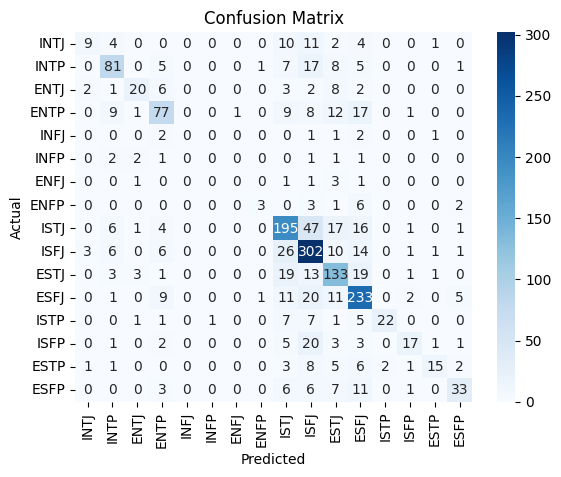
\includegraphics[width=0.8\linewidth]{images/confusion.png}}
\end{figure}

\begin{figure}[htbp]
 % Caption and label go in the first argument and the figure contents
 % go in the second argument
\floatconts
  {fig:two}
  {\caption{Feature importance analysis for LR model}}
  {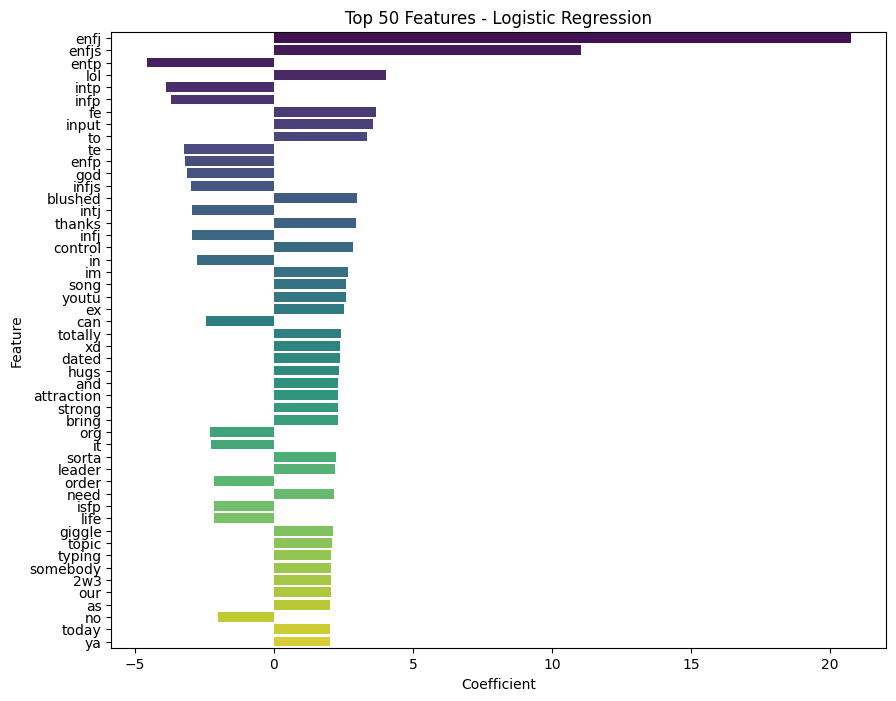
\includegraphics[width=0.8\linewidth]{images/features.png}}
\end{figure}

\newpage
\section{References}

\begin{verbatim}
    J, M. (2017). (MBTI) Myers-Briggs Personality Type | Kaggle. 
    Accessed 8 December 2023 

    K-Nearest Neighbor(KNN) algorithm. (2023, November 9). GeeksforGeeks.
    GeeksforGeeks. https://www.geeksforgeeks.org/k-nearest-neighbours/.
    Accessed 8 December 2023 

    Silva, J. (2023). COMP 562 Lecture 5. COMP 562- University of North
    Carolina at Chapel Hill. 

    Silva, J. (2023). COMP 562 Lecture 7. COMP 562- University of North
    Carolina at Chapel Hill. 

    Silva, J. (2023). COMP 562 D-Trees Lecture 3. COMP 562- University of
    North Carolina at Chapel Hill. 
\end{verbatim}


\end{document}
